\documentclass{article}
\usepackage{amsmath}
\usepackage{amssymb}
\usepackage{graphicx}
\usepackage{hyperref}
\usepackage[version=4]{mhchem}


\begin{document}
\section*{Problem}
In \(\triangle A B C\), the angle bisectors of \(\angle B, \angle C\) meet at \(T\), and the exterior angle bisectors of \(\angle B, \angle C\) meet at \(P\). Find \(\angle B P C\) if \(\angle A=\) \(72^{\circ}\).\\
\centering
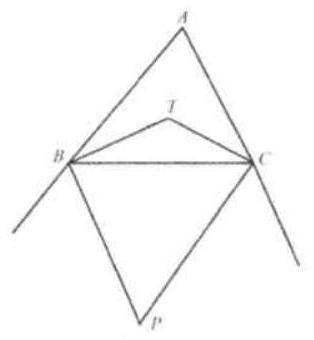
\includegraphics[width=\textwidth]{images/208(1).jpg}


\(\angle E F I=\angle E A I=\alpha\) (they face the same arc \(E I)\).\\
\(\angle F E I=\angle F A I=\alpha\) (they face the same arc \(F I)\).

In \(\triangle F E I, \angle F I E=180^{\circ}-2 \alpha=180^{\circ}-\angle A\)\\
But \(\angle F D E=\frac{1}{2} \angle F I E\). So \(\angle F D E=90^{\circ}-\frac{1}{2} \angle A\).

\section*{Solution}
\(54^{\circ\).}
Label \(\angle T B C=\angle T B A=\alpha, \angle T C B=\angle T C A=\beta, \angle C B P=\) \(\gamma\).\\
Since \(2 \alpha+2 \gamma=180^{\circ}, \alpha+\gamma=90^{\circ}\).\\
Thus \(\angle T B P=90^{\circ}\).\\
Similarly, \(\angle T C P=90^{\circ}\).\\
So points \(B, P, C\), and \(T\) are concyclic and \(T P\) is the diameter of the circle.\\
Therefore, \(\angle B P T=\angle T C B=\beta, \angle C P T=\angle T B C=\alpha\).\\
\centering
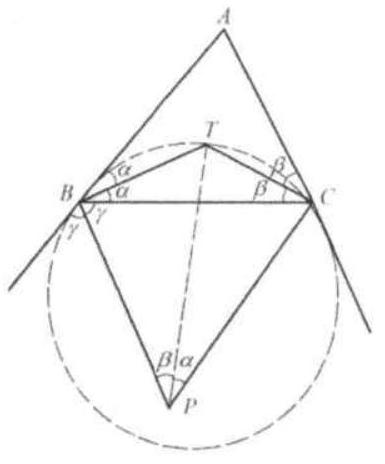
\includegraphics[width=\textwidth]{images/213(1).jpg}\\
\(\angle B P C=\alpha+\beta=\frac{\left(180^{\circ}-\angle A\right)}{2}=\frac{\left(180^{\circ}-72^{\circ}\right)}{2}=54^{\circ}\).

A
acute angle, 121\\
acute triangle, 31\\
alternate interior angles, 81, 94, 99, 107, 129, 164, 165\\
angle, \(5,3,7,11,16,17,34,35,40,47,49,50\), \(51,52,53,54,55,57,58,60,61,62,63,64\), \(65,66,67,68,71,74,84,87,106,107,124\), \(125,127,131,134,140,144,145,148,156\), \(157,159,161,162,191,192,193,196,198\), 202, 203, 204, 205, 207\\
angle bisector, 58\\
arc, \(146,148,154,160,161,162,164,168,169\), 170, 171, 191, 192, 199, 203, 204, 205, 206, 208\\
area, \(3,4,6,9,10,13,14,36,70,73,74,76,79\), \(82,84,85,86,87,89,90,91,96,104,118\), \(124,126,147,148,149,163,164,167,170\), \(173,174,179,181,183,184,194,196,199\)

B
base, \(4,10,13,70,88,129\)\\
bisect, \(2,20,26,29,37,38,44,117,129,137\), 156

C
center, \(143,145,146,147,152,153,156,163\), 167, 177, 182, 198, 199, 204, 207, 208\\
central angle, 148,154\\
chord, \(143,147,149,151,152,156,163,167\), 174, 175, 181, 182, 185, 189, 201, 206\\
circle, 143, 144, 145, 146, 147, 148, 149, 151, \(152,153,154,155,156,157,160,161,162\), \(163,164,166,167,168,169,172,173,174\), \(175,176,177,178,179,181,182,183,184\),

185, 187, 188, 189, 191, 192, 193, 199, 201, 203, 204, 205, 206, 207, 208, 209\\
circumference, 145, 159, 161, 167, 203, 209\\
collinear, 175\\
common fraction, 124, 125\\
congruent, 19, \(24,50,51,55,56,63,65,75,85\), \(90,97,130,159,175,176,177,179,182,188\), 196, 198\\
convex, \(34,37,38,40,41,42,125\)

D
decimal, 199\\
diagonal, 12, 78, 79, 85, 97, 125, 129, 179\\
diameter, \(144,145,148,149,151,152,153,159\), \(160,161,162,163,166,167,168,169,170\), \(175,179,182,187,191,192,198,199,201\), 207, 209\\
divisible, 82, 87

E
equation, \(66,68,78,93,208\)\\
equidistant, 49, 172, 202, 208\\
equilateral, \(3,41,47,79,86,94,148,173,181\), 209\\
equilateral triangle, \(3,41,47,79,86,94,148\), 173, 181, 209

F
face, \(145,146,160,161,162,164,165,168,169\), 170, 171, 191, 192, 204, 205, 206\\
formula, 24, 27, 58, 93, 178, 189, 207\\
fraction, 124, 125

G
GCF, 16

H
hexagon, 181, 184\\
hypotenuse, \(2,5,11,12,15,20,43,70,71,72\), \(79,84,85,153,158,166,170,191\)\\
inequality, 21, 25, 34, 44, 45, 53\\
inscribed angle, 148, 154, 159\\
integer, 20, 23\\
integers, 61, 62, 82, 87, 115, 118, 119, 124, 126\\
intercepted arc, 159\\
intersection, \(9,11,13,32,61,79,103,104,119\), \(120,123,124,127,152,195,196,208\)\\
isosceles, \(3,4,5,7,8,10,14,15,16,17,36,46\), \(47,53,56,57,62,71,72,73,75,80,86,87\), \(90,92,93,94,95,98,107,144,160,161,164\), 165, 191, 193, 194, 204, 206\\
isosceles triangle, \(3,4,5,7,10,14,15,16,17\), \(36,47,53,56,57,80,87,92,93,95,98,107\), 144, 160, 161, 191, 193, 194, 204, 206

L
line, 5, 1, 10, 11, 28, 29, 34, 51, 63, 66, 75, 76, \(77,79,82,85,86,87,90,92,97,99,108,114\), \(119,121,126,129,130,136,139,143,152\), 159, 172, 174, 178, 182, 184, 199\\
line segment, \(1,28,34,75,79,97,139,152,159\), 172, 199

M\\
median, \(1,2,3,4,5,7,8,9,10,14,15,16,17\), \(18,19,20,21,22,23,24,27,30,31,33,36\), \(43,46,47,61,77,78,84,93,98,115,123\), 126, 135, 148, 149\\
median of a triangle, 1, 19, 27\\
midpoint, \(1,4,8,9,10,11,12,17,18,20,22,23\), \(29,30,31,32,33,34,35,36,38,39,40,41\),\\
\(43,44,45,46,47,51,54,56,60,61,62,63\), \(64,65,72,73,82,86,88,93,98,99,103,105\), \(113,115,120,123,124,125,126,128,130\), \(131,149,174,185\),궴 \(192,194,201\)

0
obtuse triangle, 10

P
parallel, \(5,9,14,28,29,40,54,66,81,94,97\), \(100,101,102,107,118,119,121,129,130\), 136, 138, 152, 153, 174, 184, 186, 201\\
parallelogram, \(7,12,18,20,22,26,33,34,37\), \(38,40,44,47,97,107,108,114,117,120\), \(126,127,128,129,135,145,164,165\)\\
perimeter, \(40,43,62,66,79,86\)\\
perpendicular, \(5,4,10,11,17,33,35,51,55,60\), \(63,64,65,75,77,78,79,82,89,90,92,93\), \(124,143,145,147,149,152,155,156,161\), 162, 167, 172, 174, 185, 191, 201, 205, 206\\
plane, 2, 198, 202\\
point, \(1,9,10,13,32,33,35,36,40,41,49,50\), \(55,56,60,61,62,65,72,76,79,81,83,85\), \(86,92,97,98,100,101,102,103,104,106\), \(108,115,116,118,120,121,123,124,126\), \(127,129,138,143,145,148,151,152,153\), \(158,159,161,167,172\),궴 \(175,177,195,196\), 198, 199, 202, 208\\
product, 189\\
Pythagorean Theorem, 5, 15, 66, 74, 75, 76, 77, \(78,80,89,91,92,156,157,173,174,176\), 177, 178, 179, 184, 185, 187, 199, 200, 209\\
Pythagorean Triple, 77

Q
quadrilateral, \(11,34,37,38,40,41,42,77,86\), \(125,126,127,129,144,146,179,188,190\), 202, 208

R
radius, \(143,144,145,147,148,152,153,156\), \(157,172,173,175,176,177,178,179,181\), \(182,183,185,187,199,204,207,208,209\)\\
ratio, \(6,9,49,51,61,71,88,103,118,119,120\), \(123,124,129,153,170,179,180,182,183\), 186, 187, 196, 209\\
ray, 49\\
rectangle, \(2,6,12,18,20,72,84,85,106,124\), 147, 174, 184\\
relatively prime, \(61,82,115,118,119,126\)\\
right angle, \(11,40,79,82,114,153,157,159\), 164, 170\\
right triangle, \(2,3,4,5,6,8,11,12,13,15,16\), \(17,18,25,32,36,40,43,47,51,70,71,72\), \(75,77,79,82,84,85,88,91,92,113,122\), \(124,131,135,147,148,153,156,157,160\), \(163,164,166,169,170,172,173,174,178\), 184, 185, 187, 191, 196, 200

S
scalene triangle, 60, 64\\
semicircle, 149, 153, 157, 159, 164, 175, 182, 198, 201, 207\\
similar, \(51,89,91,97,100,101,102,103,105\), \(119,120,131,138,164,165,169,170,171\), 196\\
solution, \(13,73,74,89,90,92,93,100,101,102\), 119, 132, 138, 177, 178, 196, 208, 209\\
square, \(3,4,10,56,76,79,82,85,87,92,152\), 179, 199\\
sum, 19, 22, 75, 93, 179

T
tangent line, 143, 145, 160, 161, 166, 172\\
transversal, 97, 129\\
trapezoid, 28, 30, 33, 41, 45, 46, 47, 70, 72, 73, \(84,86,89,94,97,113,114,125,140,149\), 153, 164, 165, 174, 184\\
triangle, \(1,2,3,4,5,6,7,8,9,10,13,14,15,16\), \(17,18,19,20,21,22,24,25,27,28,29,30\), \(31,32,34,36,37,38,40,43,44,45,49,51\), \(53,55,56,57,60,61,62,64,65,66,70,71\), \(72,73,74,78,79,80,82,83,84,85,86,87\), \(88,89,90,91\),궴 \(95,96,97,98,103,104,107\), \(115,118,121,123,124,125,126,129,131\), \(138,144,147,151,156,157,158,159,160\), \(162,166,170,173,174,181,184,193,194\), 196, 198, 199, 201, 204, 209\\
trisect, 77, 115

V
vertex, \(1,49,79,85,126,147,153,157\)\\
vertical angles, 16, 54, 64, 99, 129, 198, 208


\end{document}

\end{document}
